PEP-II $e^- e^+$ collider utilizes PEP-II as the storage ring and SLAC linac as
the injector.
% Talk about PEP-II and its asymmetrical beam energies
In PEP-II, the $B$ mesons are produced exclusively in the following process:
$e^- e^+ \rightarrow \Y4S/ \rightarrow B \overline{B}$.
PEP-II is an asymmetrical accelerator: The $e^-$ beam is boosted to \SI{9}{GeV},
whereas the $e^+$ beam \SI{3.1}{GeV}.
The beam energies are tuned so that the invariant mass is at \Y4S/ resonance;
at the same time, the momentum of the \Y4S/ in the lab frame is
non-zero \cite{Harrison:1998yr}.

This eliminates almost all fragmentation products, reducing combinatorial
background.
Also, since the momenta of $e^- e^+$ is known, with the reconstruction of the
momentum of one $B$ meson, the rest frame of the other $B$ is
known \cite{Harrison:1998yr}.
This makes differentiating between signal ($\tau$ decay) and normalization
($\mu$ decay) easier.

% Talk about subdetectors
\BaBar/ is a barrel detector (shown in \autoref{fig:babar_detector_view})
consists of five subdetectors (from inside out):
Silicon Vertex Tracker (SVT) and Drift Chamber (DCH), which measure the momenta
and angles of charged particles.
Detector of Internally Reflected Cerenkov radiation (DIRC), together with SVT
and DCH, identifies charged particles of different masses by Cerenkov ring-
imaging and ionization energy loss of these particles.
Caesium Iodide Electromagnetic Calorimeter (EMC), which measures energy and
position of electromagnetic showers generated by electrons and photons.
A superconducting solenoid with a \SI{1.5}{T} magnetic field surrounding the
EMC, together with Instrumented Flux Return (IFR), is used to identify muons and
some neutral hadrons \cite{Lees:2013uzd}.

\begin{figure}[ht]
    \centering
    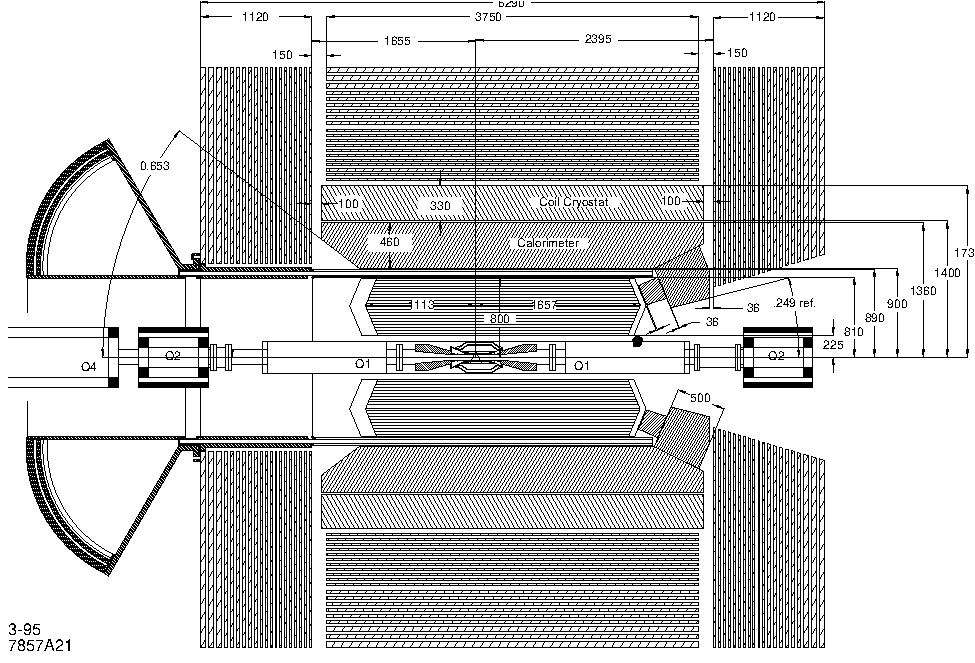
\includegraphics[width=0.7\textwidth]{figs/babar_detector_view.pdf}
    \caption{
        View of the \BaBar/ detector.
    }
    \label{fig:babar_detector_view}
\end{figure}

% Talk about BaBar being 4 pi
The distribution of angular cross section is less
polarized \cite{Boutigny:1995ib,McGregor:2008ek}, thus the detector needs to
cover almost all solid angles (a $4\pi$ detector).
Indeed, \BaBar/ has tracking coverage of 0.92, namely 92\% of the $4\pi$ solid
angle \cite{Harrison:1998yr}.

% Talk about tracking and calorimeters
$B$ physics requires excellent vertex resolution and tracking, because the two
$B$ mesons produced by \Y4S/ must be reliably separated.
\BaBar/ has excellent tracking for charged particles, and sufficient spatial
resolution in the electromagnetic calorimeter to reconstruct tracks of neutral
particles \cite{Harrison:1998yr}.
The energy resolution of the calorimeters is also sufficient \cite{Bauer:2005}.

% Talk about luminosity
\BaBar/ collected data from 1999 to 2008. Its integrated luminosity for \Y4S/
reached $424.18 \pm 0.04 \pm 1.82$~\si{fb^{-1}} on-resonance.
This resulted in $(464.8 \pm 2.8) \times 10^6$ $B \overline{B}$
events \cite{Lees:2013rw}.
